\documentclass{standalone}
\usepackage{tikz}
\usetikzlibrary{arrows, positioning}

\tikzset{
    mybox/.style={rectangle, minimum width=1cm, minimum height=1cm, draw, thick},
    myarrow/.style={thick,-latex'}
}

\begin{document}
    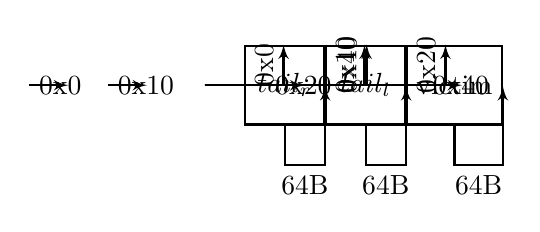
\begin{tikzpicture}[node distance=0mm]

        \draw[myarrow] (-3.25,0) node[right]{\shortstack[l]{$0$x$0$}} -- (-2.75,0);
        \draw[myarrow] (-2.25,0) node[right]{\shortstack[l]{$0$x$10$}} -- (-1.75,0);
        \draw[myarrow] (-0.25,0) node[right]{\shortstack[l]{$0$x$20$}} -- (0.25,0);
        \draw[myarrow] (1.75,0) node[right]{\shortstack[l]{$0$x$40$}} -- (2.25,0);

        \node[mybox] (TL) {$tail_r$};
        \node[mybox, right =of TL] (TL2) {$tail_l$};
        \node[mybox, right =of TL2] (V) {victim};

        \draw[myarrow] (TL.west) -- ++(-0.5,0) -| node[auto=false,pos=0.75,above,sloped]{$0$x$0$} ([shift={(0.5,0)}]TL.north west);
        \draw[myarrow] (TL2.west) -- ++(-0.5,0) -| node[auto=false,pos=0.75,above,sloped]{$0$x$10$} ([shift={(0.5,0)}]TL2.north west);
        \draw[myarrow] (V.west) -- ++(-0.5,0) -| node[auto=false,pos=0.75,above,sloped]{$0$x$20$} ([shift={(0.5,0)}]V.north west);
        \draw[myarrow] (TL2.east) -- ++(0.5,0) -| node[auto=false,pos=0.75,above,sloped]{$0$x$40$} ([shift={(-0.5,0)}]TL2.north east);

        \draw[myarrow] (TL.south) -- ++(0,-0.5) -| node[auto=false,pos=0.25,below,sloped]{$6$4B} ([shift={(0,0.5)}]TL.south east);
        \draw[myarrow] (TL2.south) -- ++(0,-0.5) -| node[auto=false,pos=0.25,below,sloped]{$6$4B} ([shift={(0,0.5)}]TL2.south east);
        \draw[myarrow] (V.south) -- ++(0,-0.5) -| node[auto=false,pos=0.25,below,sloped]{$6$4B} ([shift={(0,0.5)}]V.south east);

    \end{tikzpicture}
\end{document}